
\documentclass{article}

\usepackage{graphicx}
\usepackage{amssymb}
\usepackage{lastpage}
\usepackage{epstopdf}
\usepackage{fancyhdr}

\newcommand{\cAuthor}{Raphael Sofaer}
\newcommand{\cTitle}{Noise in an 8 Neuron Clione CPG Simulation}
\pagestyle{fancy}
\lhead{\cAuthor}                                                 %
\rhead{\cTitle}  %
\lfoot{\lastxmark}                                                      %
\cfoot{}                                                                %
\rfoot{Page\ \thepage\ of\ \pageref{LastPage}}                          %
\renewcommand\headrulewidth{0.4pt}                                      %
\renewcommand\footrulewidth{0.4pt}        

\title{\cTitle}
\author{\cAuthor}
\begin{document}
\maketitle

\section*{Introduction}
In his book Spikes, Decisions and Actions (SDA), Wilson presents an 8 neuron
model of swimming in Clione based on the work of Satterlie and Spencer (1985).
The model is two connected instances (dorsal and ventral) of a 4-neuron system.
The two sides have an inhibitory connection to each other, and a spike on one side
generates an inhibitory pulse on the other side, then a post-inhibitory rebound
sufficient to trigger a spike, generating a stable out-of-phase pattern of spikes.\\

\scalebox{0.6}{\input{Normal.tex}}
With no initial stimulus, the system remains in a stable rest state.\\
\scalebox{0.6}{\input{Rest.tex}}


Below, we examine the effect of noise on this model, determining the 
level of noise at which the characteristic out of phase synchrony is no longer stable,
the level of noise at which the system is no longer stable at rest,
and examining the other regimes which emerge as the system becomes noisy.

\section*{Methods}
All simulations were run in GNU Octave, using a version of the Clione.m included
in SDA modified for flexibility, to include noise, and to use Forward Euler integration.
Noise was generated by first generating Gaussian white noise, then filtering it to 
correspond to a $1/f^x$ ``pink noise'' pattern.\\
\scalebox{0.6}{\input{Noise.tex}}
Two grid searches were executed, varying the strength of the inibitory connection between
the dorsal and ventral sides of the model, and the intensity of the noise.
The first search used an initial stimulus of 0.5, and measured where the out-of-phase Clione
CPG remained stable.  The second used no initial stimulus, and measured the number of spikes
in the resulting time series - an estimate of where the rest state of the system remained stable.
We then sampled different areas of the resulting heat maps to examine the behavior of the system
with specific connection strengths and levels of noise.

\section*{Results}
The first grid search showed that the out-of-phase pattern is stable at relatively high levels
of noise for weak connection strengths, but as the strength of the inhibitory connection increases,
the system becomes more sensitive to noise.  In reality, the pattern persists into the blue areas
on this contour map, but the sensitivity of the method used to classify the results of the simulation
meant that slight disruptions to the pattern were classified as 'broken'.\\
\scalebox{0.6}{\input{WideHeatMap.tex}}

Above the region of out-of-phase firing, the second grid search shows that the system was not at rest,
but was either slightly disrupted or not displaying out-of-phase behaviour.  Below, we can see where
spontaneous firing begins in the absence of a stimulus.\\
\scalebox{0.6}{% GNUPLOT: LaTeX picture with Postscript
\begingroup
  \makeatletter
  \providecommand\color[2][]{%
    \GenericError{(gnuplot) \space\space\space\@spaces}{%
      Package color not loaded in conjunction with
      terminal option `colourtext'%
    }{See the gnuplot documentation for explanation.%
    }{Either use 'blacktext' in gnuplot or load the package
      color.sty in LaTeX.}%
    \renewcommand\color[2][]{}%
  }%
  \providecommand\includegraphics[2][]{%
    \GenericError{(gnuplot) \space\space\space\@spaces}{%
      Package graphicx or graphics not loaded%
    }{See the gnuplot documentation for explanation.%
    }{The gnuplot epslatex terminal needs graphicx.sty or graphics.sty.}%
    \renewcommand\includegraphics[2][]{}%
  }%
  \providecommand\rotatebox[2]{#2}%
  \@ifundefined{ifGPcolor}{%
    \newif\ifGPcolor
    \GPcolorfalse
  }{}%
  \@ifundefined{ifGPblacktext}{%
    \newif\ifGPblacktext
    \GPblacktexttrue
  }{}%
  % define a \g@addto@macro without @ in the name:
  \let\gplgaddtomacro\g@addto@macro
  % define empty templates for all commands taking text:
  \gdef\gplbacktext{}%
  \gdef\gplfronttext{}%
  \makeatother
  \ifGPblacktext
    % no textcolor at all
    \def\colorrgb#1{}%
    \def\colorgray#1{}%
  \else
    % gray or color?
    \ifGPcolor
      \def\colorrgb#1{\color[rgb]{#1}}%
      \def\colorgray#1{\color[gray]{#1}}%
      \expandafter\def\csname LTw\endcsname{\color{white}}%
      \expandafter\def\csname LTb\endcsname{\color{black}}%
      \expandafter\def\csname LTa\endcsname{\color{black}}%
      \expandafter\def\csname LT0\endcsname{\color[rgb]{1,0,0}}%
      \expandafter\def\csname LT1\endcsname{\color[rgb]{0,1,0}}%
      \expandafter\def\csname LT2\endcsname{\color[rgb]{0,0,1}}%
      \expandafter\def\csname LT3\endcsname{\color[rgb]{1,0,1}}%
      \expandafter\def\csname LT4\endcsname{\color[rgb]{0,1,1}}%
      \expandafter\def\csname LT5\endcsname{\color[rgb]{1,1,0}}%
      \expandafter\def\csname LT6\endcsname{\color[rgb]{0,0,0}}%
      \expandafter\def\csname LT7\endcsname{\color[rgb]{1,0.3,0}}%
      \expandafter\def\csname LT8\endcsname{\color[rgb]{0.5,0.5,0.5}}%
    \else
      % gray
      \def\colorrgb#1{\color{black}}%
      \def\colorgray#1{\color[gray]{#1}}%
      \expandafter\def\csname LTw\endcsname{\color{white}}%
      \expandafter\def\csname LTb\endcsname{\color{black}}%
      \expandafter\def\csname LTa\endcsname{\color{black}}%
      \expandafter\def\csname LT0\endcsname{\color{black}}%
      \expandafter\def\csname LT1\endcsname{\color{black}}%
      \expandafter\def\csname LT2\endcsname{\color{black}}%
      \expandafter\def\csname LT3\endcsname{\color{black}}%
      \expandafter\def\csname LT4\endcsname{\color{black}}%
      \expandafter\def\csname LT5\endcsname{\color{black}}%
      \expandafter\def\csname LT6\endcsname{\color{black}}%
      \expandafter\def\csname LT7\endcsname{\color{black}}%
      \expandafter\def\csname LT8\endcsname{\color{black}}%
    \fi
  \fi
  \setlength{\unitlength}{0.0500bp}%
  \begin{picture}(11520.00,8640.00)%
    \gplgaddtomacro\gplbacktext{%
      \colorrgb{0.00,0.00,0.00}%
      \put(797,4470){\rotatebox{90}{\makebox(0,0){\strut{}k (connection strength)}}}%
      \colorrgb{0.00,0.00,0.00}%
      \put(5068,450){\makebox(0,0){\strut{}Noise level: mean mV}}%
      \csname LTb\endcsname%
      \put(5068,8291){\makebox(0,0){\strut{}Spikes generated in the absence of stimulus}}%
    }%
    \gplgaddtomacro\gplfronttext{%
      \colorrgb{0.00,0.00,0.00}%
      \put(1377,950){\makebox(0,0)[r]{\strut{}0}}%
      \colorrgb{0.00,0.00,0.00}%
      \put(1377,2124){\makebox(0,0)[r]{\strut{}100}}%
      \colorrgb{0.00,0.00,0.00}%
      \put(1377,3297){\makebox(0,0)[r]{\strut{}200}}%
      \colorrgb{0.00,0.00,0.00}%
      \put(1377,4471){\makebox(0,0)[r]{\strut{}300}}%
      \colorrgb{0.00,0.00,0.00}%
      \put(1377,5644){\makebox(0,0)[r]{\strut{}400}}%
      \colorrgb{0.00,0.00,0.00}%
      \put(1377,6818){\makebox(0,0)[r]{\strut{}500}}%
      \colorrgb{0.00,0.00,0.00}%
      \put(1377,7991){\makebox(0,0)[r]{\strut{}600}}%
      \colorrgb{0.00,0.00,0.00}%
      \put(1497,750){\makebox(0,0){\strut{}0}}%
      \colorrgb{0.00,0.00,0.00}%
      \put(3227,750){\makebox(0,0){\strut{}0.0005}}%
      \colorrgb{0.00,0.00,0.00}%
      \put(4958,750){\makebox(0,0){\strut{}0.001}}%
      \colorrgb{0.00,0.00,0.00}%
      \put(6688,750){\makebox(0,0){\strut{}0.0015}}%
      \colorrgb{0.00,0.00,0.00}%
      \put(8419,750){\makebox(0,0){\strut{}0.002}}%
    }%
    \gplgaddtomacro\gplbacktext{%
    }%
    \gplgaddtomacro\gplfronttext{%
      \colorrgb{0.00,0.00,0.00}%
      \put(10187,950){\makebox(0,0)[l]{\strut{}0}}%
      \colorrgb{0.00,0.00,0.00}%
      \put(10187,2564){\makebox(0,0)[l]{\strut{}5}}%
      \colorrgb{0.00,0.00,0.00}%
      \put(10187,4177){\makebox(0,0)[l]{\strut{}10}}%
      \colorrgb{0.00,0.00,0.00}%
      \put(10187,5791){\makebox(0,0)[l]{\strut{}15}}%
      \colorrgb{0.00,0.00,0.00}%
      \put(10187,7404){\makebox(0,0)[l]{\strut{}20}}%
    }%
    \gplbacktext
    \put(0,0){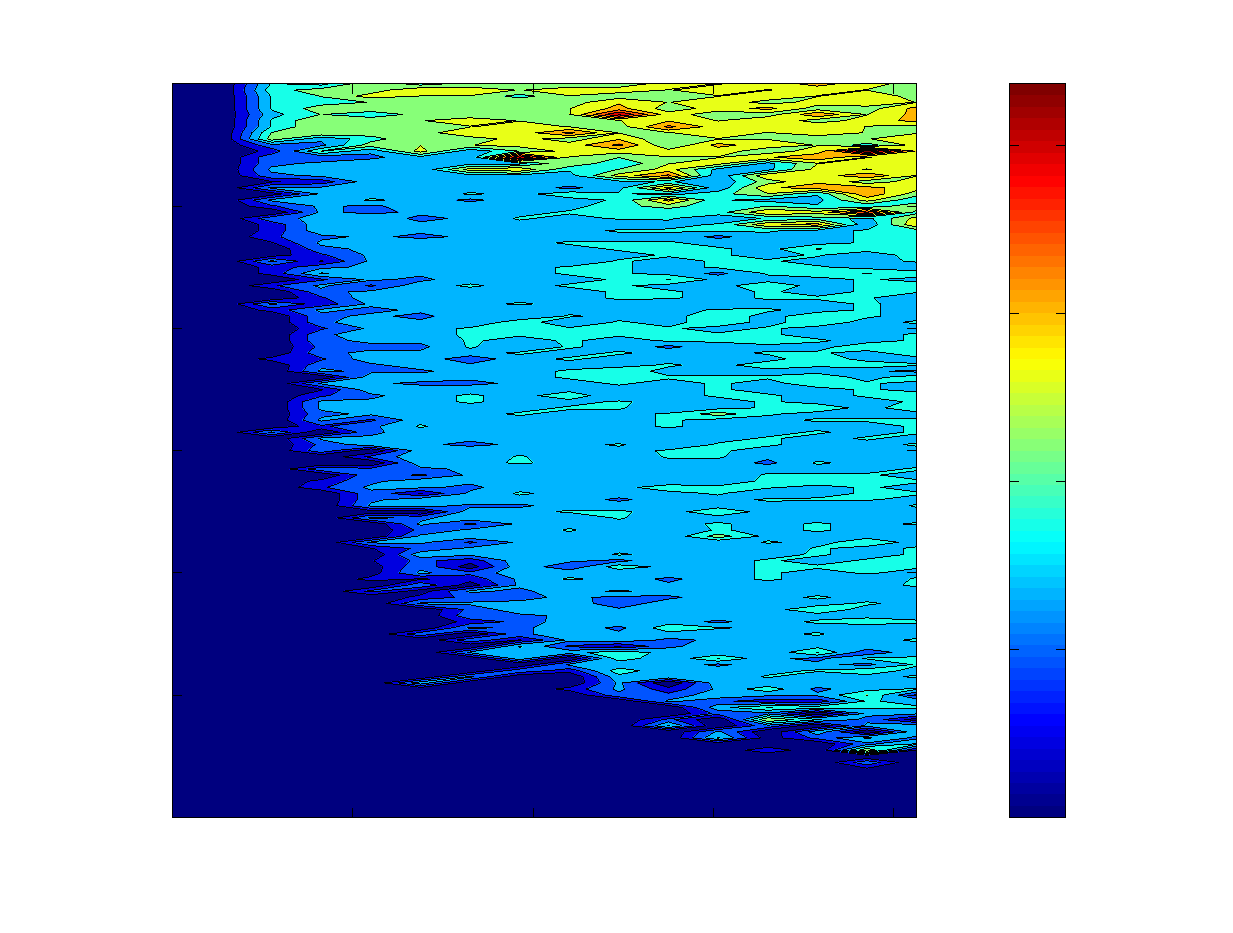
\includegraphics{nSpikesHeatMap}}%
    \gplfronttext
  \end{picture}%
\endgroup
}

We can see from the two contour maps added together (so the color is essentialy meaningless except
as on or off), that the strict stability of out-of-phase firing ends significantly before spontaneous 
firing begins.\\
\scalebox{0.55}{\input{ComHeatMap.tex}}

With slight noise the system is basically unaffected by the noise, and the out-of-phase pattern
is not visibly different.\\
\scalebox{0.6}{\input{NormalSlightNoise.tex}}

With more noise, but not enough to cause spontaneous firing, the out-of-phase firing equilibrium
is still there, but the noise is sufficent to kick the system to rest. \\
\scalebox{0.55}{\input{DisruptedTurningOff.tex}}

At a higher connection strength, we occasionally see spikes that seem to have been suppressed by
the simultaneous firing of the other neuron.\\
\scalebox{0.6}{\input{SupressedSpikes.tex}}

With no stimulus and a high connection strength, we can see a little bit of out-of-phase subthreshold
activity, even when there is not enough connectivity or noise to cause action potentials.\\
\scalebox{0.6}{\input{SubthresholdOutOfPhase.tex}}

At very levels of high inhibitory gain, we see a competition regime, where one neuron spikes steadily
until noise knocks it into subthreshold activity and the other neuron starts spiking.\\
\scalebox{0.6}{\input{Competition.tex}}

At high levels of noise, the noise starts to overcome the inhibitory connection, and while the 
neurons remain synchronized, occasionally they fire at the same time.\\
\scalebox{0.6}{\input{Simultaneous.tex}}
\section*{Conclusions}
The simplified Clione model that Wilson puts forward in SDA does not show many of the behaviours in
Satterlie's paper, but the central pattern of out-of-phase firing is fairly robust to noise.
As the pattern is overcome by rising levels of noise, the connections between the neurons
maintain some synchrony between the dorsal and ventral sides.  First the pattern is disrupted by noise,
then noise allows alternate regimes like competition to appear, and finally the pattern breaks down
with consistent simultaneous firing.  When the pattern does break down,
this simple CPG model could be a useful way to show that small amounts of noise, too small to see in
a graph, can create qualitatively very different results.
\end{document}
